%% $Id: main.tex,v 1.12 2001/08/16 18:01:42 pwaddell Exp $

%\documentclass{article}
\documentclass{elsart}
% \usepackage{times}
\usepackage{graphicx}
\usepackage{natbib}
\usepackage{url}

\topmargin -0.5in
\oddsidemargin  0 in
\evensidemargin  0 in
\textwidth   6.5 in
\textheight 9 in

\setlength{\parindent}{0.0in}
\setlength{\parskip}{7pt plus 1pt}
\newcommand{\tight}{\itemsep 0pt}

\newcommand{\code}[1]{{\small \texttt{#1}}}
\newcommand{\email}[1]{{\texttt{#1}}}

% Programming language keywords
\newcommand{\keyw}[1]{{\bf #1}}

% Variable names, defined with separate style to facilitate customization
\newcommand{\varnm}[1]{{\textsf{#1}}}


\sloppy

\begin{document}

\begin{frontmatter}
%% $Id: title.tex,v 1.12 2001/08/18 00:56:25 borning Exp $
%% Title information

\title{An Extensible, Modular Architecture for Simulating Urban
Development, Transportation, and Environmental Impacts}
\author{Michael Noth}
\renewcommand{\thefootnote}{\fnsymbol{footnote}}
\setcounter{footnote}{0} \hspace{-7.5mm} \footnote{Corresponding
author}
%\renewcommand{\thefootnote}{\arabic{footnote}}
\author{Alan Borning}
\address{Dept.\ of Computer Science \& Engineering,
University of Washington, \\
Box 352350,
Seattle, Washington 98195,
\{noth,borning\}@cs.washington.edu}
\author{Paul Waddell}
\address{Evans School of Public Affairs,
University of Washington, \\
Box 353055, Seattle, Washington 98195,
pwaddell@u.washington.edu}

\renewcommand{\thefootnote}{\arabic{footnote}}
\setcounter{footnote}{0}

%\begin{tabular}{cc}
%Michael Noth and Alan Borning        &    Paul Waddell \\
%Dept.\ of Computer Science \& Engineering  & Evans School of Public Affairs \\
%University of Washington, Box 352350 &  University of Washington, Box 353055 \\
%Seattle, Washington 98195 &  Seattle, Washington 98195 \\
%\{noth,borning\}@cs.washington.edu  & pwaddell@u.washington.edu
%\end{tabular}
%}

%\maketitle

%{\large\bf\em Draft.}  \emph{We have submitted this paper for
%journal publication --- comments and suggestions are most
%welcome!}

% LocalWords:  noth Waddell Exp pwaddell Borning

\newpage
%% $Id: abstract.tex,v 1.9 2001/08/18 00:56:25 borning Exp $

%\subsection*{Abstract}
\begin{abstract}

UrbanSim simulates the development of urban areas, including land
use, transportation, and environmental impacts, over periods of
twenty or more years.  Its purpose is to aid urban planners,
residents, and elected officials in evaluating the long-term
results of alternate plans, particularly as they relate to such
issues as housing, business and economic development, sprawl, open
space, traffic congestion, and resource consumption.  From a
software perspective, it is a large, complex, system, with heavy
demands for excellent space efficiency and support for software
evolution.  It consists of a collection of models that represent
different urban actors and processes, an object store that holds
the state of the simulated urban environment, a model coordinator
that schedules models to run and notifies them when data of
interest has changed, and a translation and aggregation layer that
performs a range of data conversions to mediate between the object
store and the models.  The paper concludes with a discussion of
the lessons learned regarding software architecture to support
rapid evolution within the field of urban simulation.

\end{abstract}

% LocalWords:  noth UrbanSim Exp borning pwaddell

\newpage
\end{frontmatter}

\newpage
%% $Id: intro.tex,v 1.19 2001/08/16 18:01:27 pwaddell Exp $

\section{Introduction}
\label{sec:introduction}

Patterns of land use and available transportation systems play a
critical role in determining the economic vitality, livability,
and sustainability of urban areas.  Transportation interacts
strongly with land use.  For example, automobile-oriented
development may induce demand for more roads and parking (which in
turn induces more automobile-oriented development), while compact
urban environments may induce more walking and demand for transit.
Both land use and transportation have significant environmental
effects, in particular on emissions, resource consumption, and
conversion of rural to suburban or urban land.

Good technical support can play an important role in fostering informed
civic deliberation and debate on these issues.  To aid urban planners,
residents, and elected officials in evaluating alternate
scenarios---packages of policies and investments---we want to simulate the
effects of these scenarios on patterns of urban growth and redevelopment,
of transportation usage, and resource consumption, over periods of twenty
or more years.

Early attempts at comprehensive urban simulations in the 1960s and
early 1970s were largely unsuccessful \citep{lee-1973,lee-1994}.
Much has changed since then, both on the supply side (including
dramatically improved hardware, theoretical and methodological
advances such as discrete choice choice modeling
\citep{mcfadden-1973,mcfadden-iatbr-2000}, and the emergence of a
commercial GIS market), and on the demand side (including public
concern over sprawl, legal challenges to transportation plans made
without considering their land use implications
\citep{garret-1996}, and regulatory requirements such as the Clean
Air Act Amendments of 1990).  As a result, there has been somewhat
of a renaissance in interest in urban simulation modeling over the
past decade.

However, in terms of planning agency practice, land use planning
is still often poorly integrated with transportation planning,
despite their strong interactions.  While transportation models
have been in routine use by metropolitan planning organizations
for decades, the state of common practice in land use modeling,
and in integrated land use and transportation modeling, is much
less advanced than that for transportation modeling alone.  For
example, the Travel Model Improvement Project sponsored by the
U.S. Department of Transportation and the Environmental Protection
Agency has focused a substantial investment on TRANSIMS, a new
traffic microsimulation model \citep{TRANSIMS-1999}, but almost no
federal investment has occurred on land use modeling to integrate
with these new travel models.

The UrbanSim system has been designed and implemented in response
to these needs.  It is a system for simulating the development of
urban areas, including land use, transportation, and environmental
impacts, over periods of twenty or more years
\citep{waddell-env-and-planning-2000,urbansim-reference-2000,waddell-nse-2001}.
From a software perspective, it is a large, complex application,
with heavy demands for excellent space efficiency and support for
software evolution. The system is fully operational and freely
available via our web site at {\sf www.urbansim.org}.  It consists
of around 130,000 lines of Java code for the core UrbanSim system;
including the visualization, data preparation, and calibration
tools, the total is approximately 200,000 lines, plus another
100,000 lines of automatically generated code.  It has been
applied to Eugene-Springfield, Oregon; Salt Lake City, Utah; and
Honolulu, Hawaii, working with the planning organizations in those
metropolitan regions.  Application to other regions is underway.
We have also done a historical validation of the system, starting
UrbanSim with 1980 data for Eugene-Springfield, running it through
1994, and comparing the results with what actually transpired
\citep{waddell-oregon-2000}.  Correlations between results of the
15 year simulation and observed data were generally above 0.8 at
the level of the grid cell, and were higher for spatial
aggregations such as traffic analysis zones.

% LocalWords:  noth UrbanSim sustainability Exp pwaddell GIS

%% $Id: relatedwork.tex,v 1.17 2001/08/18 01:15:58 borning Exp $

\section{Related Work}
\label{sec:relatedwork}

There is a huge body of work on urban transportation modeling,
land use modeling, and integrated land use/transportation
modeling.  Reviews and assessments of existing systems are given in
references
\citet{dowling-nchrp-2000,epa-report-2000,miller-tcrp-1999,parsons-1998,southworth-1995},
among others. Considerable progress has recently been made in land
use modeling in both experimental and deployed systems. However,
except for UrbanSim, all the operational models in use by planning
agencies rely on a cross-sectional, aggregate, equilibrium
approach.  Such models include DRAM/EMPAL
\citep{putman-book-1983}, TRANUS \citep{delabarra-book-1995},
MEPLAN \citep{echenique-transport-reviews-1990}, METROSIM
\citep{anas-book-1994}, and 5-LUT
\citep{martinez-env-planning-1992}.  The cross-sectional,
equilibrium framework implies that there are no relevant temporal
dynamics to the processes of urban change; rather, one can model
urban development as a static process that represents an economic
or a transportation optimization problem.  In other words, these
models could be run for the year 2050 without needing to model the
dynamics of evolution between the current time and the year 2050.
Clearly, this is a severe simplification, and makes problematic
the potential integration of these models with models of dynamic
environmental processes, or even of the dynamic evolution of human
behavior with respect to the built environment.  The approach
taken in UrbanSim more closely compares to the dynamic
disequilibrium HUDS model \citep{kain-book-1985} and the DORTMUND
microsimulation model
\citep{wegener-dortmund-1983,wegener-spiekermann-1996}, but
differs from these in having substantially greater spatial detail
and incorporating the nonresidential dimensions of urban
development.

% omitted for new journal:
% Reference \cite{beimborn-1996} is a short, useful introduction to the area
% for the nonspecialist.

Another substantial body of related work concerns Integrated
Assessment Models (IAMs), which model the interactions between
human and ecological systems in an integrated way.  A major
motivation for models of this kind is the assessment of global
environmental change
\citep{alberti-envplanning-1999,dowlatibadi-1995,parson-1995,rotmans-1995,weyant-1996}.
While the first generation of operational IAMs has emerged in the
mid-eighties, their roots can be traced back to earlier modeling
work in the late sixties and early seventies
\citep{forrester-book-1971,isard-1969,meadows-book-1982,odum-book-1983}.
Not surprisingly, all of these global-scale models are quite
aggregate, predicting environmental disturbances from broad
measures of economic growth and urbanization.  The UrbanSim
approach, by contrast, uses substantial spatial detail, and a
clearer behavioral approach grounded in discrete-choice theory.

In addition to global models, spatially-explicit regional integrated models
are now emerging, such as the Patuxent Landscape Model
\citep{voinov-envmodeling-1999}.  The Patuxent Landscape Model contains an
economic land use conversion model that uses a statistical process to
determine probabilities that grid cells will be allocated to forest,
agricultural, or urban usage.  The resulting conversion probabilities are
used to predict land use patterns which determine the land cover values
used as an input to the PLM's hydrology component.  Communication between
the land conversion and hydrology models is implicit through changed data
values in grid cells.  Several of the factors used in its land use
conversion component are similar to ones used in UrbanSim (e.g., access to
infrastructure, historical tax assessor data), but UrbanSim explicitly
models agents and their actions rather than using statistical or
finite-element processes.

Finally, another area of related work concerns agent-based
modeling, artificial life, and cellular automata.  In agent-based
modeling in its pure form, individual agents and their actions are
simulated, with each agent having local knowledge; global behavior
then emerges from these agent-level interactions.  Agent-based
modeling has been used for a wide range of applications, including
economic, sociological, biological, and physical simulations.  Two
that are closely related to UrbanSim are Sugarscape
\citep{epstein-book-1996,sugarscape-web}, a simulation of a small,
artificial society, and Aspen, a microanalytic simulation of the
entire U.S. economy \citep{pryor-sandia-1996,sandia-aspen-web}.
These approaches attempt to produce plausible macro-level behavior
as emergent properties of micro-level behavior.  This approach has
not yet evolved to the point of operational use in applied
planning settings, but represents a significant area of ongoing
research.

Cellular automata have been used for simulating urban development
\citep{batty-envplanning-1998,batty-computers-environment-1999,clark-envplanning-1997},
as well as for other applications such as simulating change in
land cover, freeway traffic, or the spread of wildfires.  In its
classic form, a cellular automaton consists of a regular array of
cells, each of which has a finite number of states.  Each state
change must be local, depending only on the states of neighboring
cells.  Urban processes, such as sprawl or urban decay, can emerge
from simple local rules.  However, these restrictions do not
always mesh well with our goal of supporting deliberation about
public policy.  For example, rather than viewing the conversion of
rural areas to urban ones as an analog of a biological process in
which the suburb grows and occupies increasingly wider areas, in
UrbanSim we view this process as the result of interactions among
the Land Developer Model (which simulates developers actively
seeking out development opportunities throughout the region in
response to market conditions, zoning regulations, taxes and
incentives, and the like), the location choice models (which
simulate residents or businesses seeking housing and commercial
space), and the Land Price Model.  More recently, researchers have
experimented with extensions of the cellular automata formalism
that incorporate extensions such as more agent-like behavior or
non-local search \citep{batty-jiang-1999,osullivan-2000}.

The UrbanSim approach assimilates aspects of these recent
developments in highly disaggregate agent-based and cellular
automata models, while retaining the flexibility to use
macro-scale model components when appropriate.  This
assimilative approach requires that the software architecture
support multiple modeling approaches, and not be optimized or
restricted to only one.  Models may be designed to operate at
different temporal and spatial scales, requiring unusual
flexibility from the software architecture. 

One 
implication of this for the software architecture is the need for a flexible
mechanism for assimilating model components and coordinating their
behaviors.  To meet this need, we use
\emph{implicit invocation},  
a software engineering technique in which different system components
communicate indirectly, rather than directly using procedure calls.  In our
realization of implicit invocation,
models communicate by registering
interest in objects and fields held in the Object Store, and by
being notified when such an object or field has been changed by
another model; but not by invoking each other explicitly.
This allows models to be developed more independently of each other.
(See Section \ref{sec:implicit-invocation} for details.)
Additional advantages and other applications of
implicit invocation are described in references
\citet{garland-aske-1993,sullivan-tse-1992,sullivan-tse-1996}.
Implicit invocation is essentially an event mechanism; related
concepts include active variables in
LOOPS~\citep{stefik-software-1986}, active databases such as
AP5~\citep{cohen-sigmod-1989}, and the Smalltalk-80
Model-View-Controller~\citep{krasner-joop-1988} and Field
integration mechanisms~\citep{reiss-book-1994}.  A discipline of
defining and using event-based programming mechanisms is
evolving~\citep{barrett-tse-1996,carzinga-saw-1998,
garlan-vdm-1991}.

The UrbanSim simulation approach, in summary, differs along
several lines from prior urban simulation models.  It is far more
disaggregate than any operational model implemented to date.  It
uses a dynamic, path-dependent approach that does not impose
simplifying assumptions of general equilibrium.  It is designed
for operational use to examine the effects of land use,
transportation, and the environmental plans and policies. And it
adopts an assimilative approach that draws from multiple streams
of ongoing research in urban simulation, including multi-agent,
cellular automata, and macro-scale models. The software
architecture described in this paper provides a modular and
extensible simulation environment that facilitates developing and
integrating urban models with varying temporal and spatial scales.

% LocalWords:  Exp UrbanSim AP Smalltalk GIS EMPAL TRANUS MEPLAN METROSIM  LUT
% LocalWords:  IAMs PLM's borning Patuxent Sugarscape wildfires StarLogo noth
% LocalWords:  aske sullivan tse stefik cohen sigmod krasner joop reiss barrett
% LocalWords:  carzinga garlan vdm tcrp southworth putman delabarra echenique
% LocalWords:  anas martinez env alberti envplanning dowlatibadi rotmans weyant
% LocalWords:  forrester isard odum voinov envmodeling epstein sugarscape pryor
% LocalWords:  sandia batty clark jiang osullivan pwaddell dowling nchrp epa
% LocalWords:  HUDS kain wegener dortmund spiekermann

%%% UrbanSim architecture figure and caption, on separate pages
%% $Id: USArchFig.tex,v 1.2 2001/05/17 18:44:20 pwaddell Exp $

\newpage
\begin{figure*}
\center
\resizebox{0.75 \textwidth}{!}{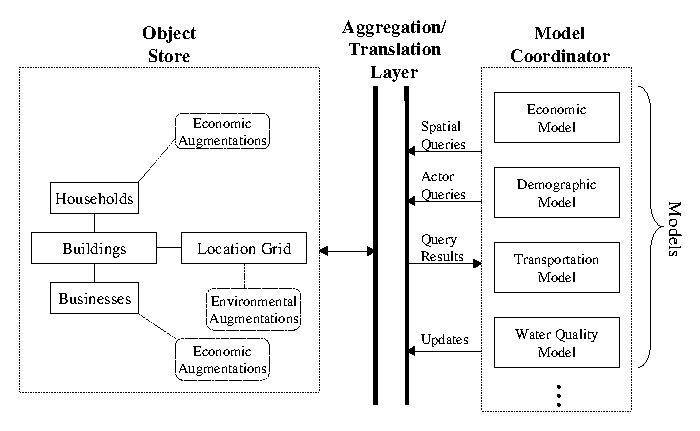
\includegraphics{USDiag1.eps}}
%\caption{UrbanSim architecture}
\label{fig:USArch}
\end{figure*}

%\clearpage
Figure~\ref{fig:USArch}: UrbanSim architecture.

%% $Id: overview.tex,v 1.17 2001/08/18 00:56:25 borning Exp $

\section{Overview of the UrbanSim Architecture}
\label{sec:overview}

To simulate an urban region, UrbanSim employs a collection of
interacting \emph{models}, representing different actors and
processes in the urban environment, such as residents, businesses,
land developers, and transportation networks.  Each model encodes
the behavior of agents in the simulation, as well as the objects
they operate upon, such as land parcels and buildings.  Objects
correlate directly with easily-identifiable objects in the real
world, making it easier to reason about their properties and
behaviors.  Agents can be shared across models, as can the objects
they operate upon.  Much more than other urban modeling systems,
the UrbanSim model is very disaggregate and has high data
requirements.  These requirements enable modeling of processes to
be done at a fine level, which allows use of detailed spatial data
in a manner not possible with more aggregate systems.  At the same
time, this makes the design and implementation of the system more
difficult from a software perspective.  Figure \ref{fig:USArch}
illustrates the software architecture of the UrbanSim system.

\begin{figure*}
\center \resizebox{0.75
\textwidth}{!}{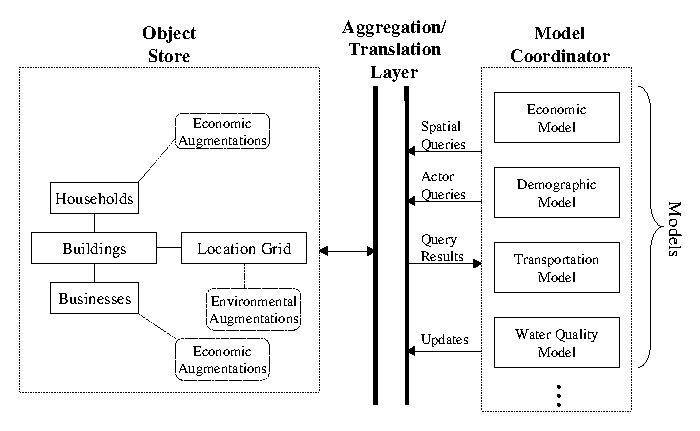
\includegraphics{USDiag1.eps}} \caption{UrbanSim
architecture} \label{fig:USArch}
\end{figure*}

%Figure~\ref{fig:USArch}: UrbanSim architecture.

In addition to the models, the other principal components of
UrbanSim are a \emph{model coordinator} that schedules models to
run and notifies them when data of interest have changed, an
\emph{object store} that holds the shared representations of
agents and other entities in the simulated world, and a
\emph{translation and aggregation layer} that performs a range of
data conversions to mediate between the Object Store and the
models.  The models do not communicate directly with each other;
rather, they communicate via shared data held in the Object Store,
mediated by the translation and aggregation layer.  This
extensible, modular architecture supports system evolution, in
particular replacing a model with a revised one, and creating and
integrating new models.  It allows models to define and share
common sets of objects that they all operate upon, via the Object
Store (regardless of the original source of the data), and also
allows them to monitor changes to data fields, providing a
convenient method for models to synchronize their actions.

A primary goal of this architecture is to move as much of the
software complexity out of the individual models and into the
supporting infrastructure as possible.  This supporting
infrastructure need be written just once, and can have the
attention of an expert programmer.  The models, on the other hand,
are both numerous and frequently changing due to rapidly evolving
theory, methods and modeling needs. Often, specifying them is
difficult, requiring considerable domain-specific expertise,
specialized data, and testing; the more one can relieve the model
designers of programming burdens the better, so that they can
concentrate on issues arising from the domain.

% LocalWords:  Exp UrbanSim USDiag eps noth borning pwaddell

\section{Models}

The model architecture is adapted from the functional design of SAM,
and also informed by the development of OPUS and UrbanSim. The
functionality in SAM focuses on the allocation of land use by
sector to grid cells, from aggregate information at a mid-level
geography such as MPAs.  By reference to the UrbanSim model system,
this functionality is approximately equivalent in purpose to the
real estate development model component of UrbanSim, with some key
differences.  UrbanSim attempts to include a complete representation
of the real estate market, with occupants (consumers: households
and jobs), buildings and land (suppliers: developers and property
owners), and prices (markets: hedonic regressions representing the
interaction of suppliers and consumers).

The architecture for the model system proposed for AZ-SMART is
based on a 3-year plan, and incorporates the complete market
representation as in UrbanSim, and a multi-level geography and
model system.  We describe this in the Full Model System subsection
 below, and then focus on a Phase 1 Model System in the subsequent
 section.

\subsection{Full Model System}
The full model system proposed for AZ-SMART involves some
hybridization and extension of elements of UrbanSim and SAM-IM.
Below we itemize the core elements of the full model system
architecture.

\begin{itemize}

\item \emph{Land-Structure-Occupant Accounting}: The full market
representation and explicit representation of and accounting of
Land-building-occupant objects and their relationship is proposed
for the full model architecture.

\item \emph{Parcels and Buildings}: Land could be represented by
parcels, land use polygons, or cells, but it is expected that
the parcel concept would be used as the principal representation
of land, and that in areas that do not have parcel data available,
land use polygons could be used in a way that treats them as
equivalent to (possibly large) parcels.  Note that there are many
to one relationships from buildings to land and from occupants to
building.  That is, a building may contain multiple occupants,
and a parcel (or land use polygon) may contain multiple buildings.
In the event that building data is not available, it could be
imputed, to preserve a consistent data model.

\item \emph{Development Projects, Sites and Templates}: Development
 Projects are proposed as a higher-level construct to represent
 one or more parcels that form a coherent single development
 project, such as single-family housing subdivision, or a shopping
 center complex.  These development projects will deal both with
 known \emph{development projects} which the user wishes to
 incorporate into the simulation, and also development projects
 predicted by the simulation and assigned to \emph{development
 sites}.  For predicted development projects, a set of pre-defined
  \emph{development templates} provide a set of configurations of
  development that include at a minimum the mix of building types
  (land uses), density, size and timetable for development.

\item \emph{Multi-level Model}: The full model system would use
a multi-level approach, incorporating parcels as the lowest level
(buildings are linked to parcels), and for the forseeable future,
one higher level geography to represent an intermediate geography
between the county and the parcel.  Traffic Analysis Zones (TAZ)
are proposed as the basis for this mid-level geography in the full
 model, simplifying the interface with the travel model system.
 There are behavioral and practical reasons for using a two-level
 geography in the model system.  Behaviorally, it is based on the
 expectation that consumers looking for a location (e.g. a household
  searching for a house) compare neighborhoods, and select properties
  to examine based on their assessment of the neighborhoods. In
  practical terms, the two-level geography provides a more convenient
  way to interface models in a modular way, for example to interface
  the travel model system, or to run the model system for corridor or
  area studies where more detail is needed in a subset of the planning
  region and less is needed outside of this focus area.

\item \emph{Microsimulation}: The proposed architecture is based on
explicit representation of the agents and objects being modeled at a
microscopic level.  Parcels, buildings, businesses (or jobs),
households, and eventually, persons (for supporting activity-based
travel models and workplace choice models and individual-level
accessibility calculations).

\item \emph{Temporal Dynamics}: The model system would be able to
use a specified time interval, such as 5-year or 1-year steps,
between which it would simulate changes to the state of each object
and agent in the system (construction of new buildings or conversion
of existing ones, movement of households and businesses from one
location to another, creation of new households or businesses).

\item \emph{Models and Interface}: A set of models will be interfaced
through a common data store, and managed by a Model Coordinator that
controls their execution and implements events (changes to the data)
proposed by models.  The individual models would be the following:

\begin{itemize}
\item Demographic Transition (Region): Reconciles the control totals
of population (by household type) with the database - adding households
to the database or removing them if a household type is declining.
\item Employment Transition (Region): Reconciles the control totals
of employment (by sector) with the database - adding businesses (jobs)
to the database or removing them if a sector is declining.
\item Development Project Transition (Region): Reconciles the total
demand for real estate by type, including the results of the Demographic
and Employment Transition models, with the existing stock of real estate,
by generating proposed Development Projects until vacancy rates reach
long-term structural levels.
\item Household Relocation (Region): Predicts whether a household will
move from their existing residence during the next time step.
\item Business Relocation (Region): Predicts whether a business  (job)
will move from their existing location during the next time step.
\item Household Location (TAZ and Parcel): Predicts the building that
a new or moving household will choose from among the set of buildings
with a vacanct unit.
\item Business Location (TAZ and Parcel): Predicts the building that a
new or moving business (job) will choose from among the set of buildings
with sufficient vacanct space.
\item Parcel Subdivision (Parcel): Predicts the number and size of
parcels to create from a large parcel that is to be subdivided to create
a development project. Depending on whether the project is known or
predicted this will use information provided in the development project
description or drawn from a development template.
\item Parcel Aggregation (Parcel): Combines adjacent parcels to create
a \emph{development site} suitable to place a development project.
\item Demolition (Building): Removes existing buildings based on age
and other characteristics that would indicate a high probability to
convert to another use or be abandoned.
\item Development Project Location (Development Site): Predicts the
development site chosen to locate a development project.
\item Building Development Model (Parcel): This would be based on the
Development Velocity Model, and predicts the construction of individual
buildings on parcels within a development project.
\item Real Estate Price Model (Building): This will predict the price
per unit (or sqft) for each type of real estate at each location (parcel).
\item Simplified Travel Model (TAZ): An abbreviated travel model with
just a.m. peak, and other simplifications to provide a relatively
high-speed regional travel model to use in intermediate years preceding
the target year for the regional transportation plan.
\end{itemize}
\end{itemize}

The models proposed for implementation in Phase 1 of this project are
described in greater detail in the following section.

\subsection{Phase 1 Model System}
Phase 1 of the AZ-SMART project focuses on the allocation of land use
sectors, essentially the real estate development process.  The plan
for Phase 1 is to focus on the real estate development components of
the full model system described in the preceding section, and to
suppress or use only simple 'stub' models for the remaining models
in the full system.  The objective is to provide the functionality
that is provided now by SAM, but in an implementation that is a
very big step towards a fully integrated market simulation model
system such as UrbanSim, and incorporating valuable innovations
such as the management of known development projects, and the use
of an intermediate level geography such as RAZ as the basis for
control totals for allocation to parcels (or land use polygons).

The following models would be the focus of model development in Phase 1:

\begin{itemize}
\item Parcel Subdivision (Parcel)
\item Parcel Aggregation (Parcel)
\item Development Project Location (Development Site)
\item Building Development Model (Parcel)
\end{itemize}

The following models would be implemented for completeness, but would
use only the simplest specification, to allow completeness.  For example,
the household location choice model could use an empty specification,
which would randomly allocate the household control total for a RAZ to
the housing units that have been developed on parcels in the RAZ.

\begin{itemize}
\item Demographic Transition (RAZ)
\item Employment Transition (RAZ)
\item Development Project Transition (RAZ)
\item Household Location (Parcel)
\item Business Location (Parcel)
\end{itemize}

The components of the full model system would be deferred until after Phase 1:

\begin{itemize}
\item Demolition (Building)
\item Real Estate Price Model (Building)
\item Simplified Travel Model (TAZ)
\end{itemize}





The model architecture has the following steps, using a 5-year time interval:

=== Determine Quantity of Development Needed ===

* Translate mid-level model predictions of population and employment by RAZ (or other mid-level geography) into predicted demands for housing units and land area of non-residential uses by type.
** This would be done using average density and occupancy assumptions.

=== Determine Development from Active Projects ===

* Compute the quantity of development expected in a RAZ (or other mid-level geography) for each land use sector, based on the velocity within Active Development projects.

* Assign the development generated by Active Development Projects to the cells within those developments.

=== Determine Eligible Development Sites ===

* Evaluate cells with vacant land to determine what kinds of development would be permitted on them according to the development constraints represented by Planned Land Use and other constraints (slopes, etc).  This applies development constraints in order to produce Eligible Vacant Lands for development.

* Evaluate potential availability of Redevelopment Districts for new development.

* Generate 'Development Sites' from 'patches' of available land suitable for development.  These are areas formed by contiguous cells eligible for development for a particular land use sector, and would serve as a counterpart to the polygons digitized by users for planned and active development projects.  They would allow the comparable representation of Development Sites from all sources.

=== Assign Development Projects to Development Sites ===

* Use 'Development Sites' as the candidate set of locations for new development within the RAZ.

* Generate a set of proposed 'Development Projects' that would fill the gap in the RAZ between the development that is generated by evaluating the velocity of Active Development Projects and the quantity required to meet the RAZ control totals.

* Compute logit model probability that a Development Project in a RAZ will choose one of the available candidate Development Sites.

** Compute variables used in utility (scoring function)
** Multiply variables by their coefficients
** Compute utility
** Compute probability

* 'Choose' a Development Site for each Development Project to be located based on the logit probabilites.  Specifically, draw a random number and compare it to the cumulative probability distribution across the alternative Development Sites.  Choose the site that the random number falls within (the choice pattern will be proportional to the logit probabilities).  Ensure that the capacities of the sites are respected: if a Development Project is too big for a site, exclude it from consideration.

* Once a Development Site is chosen for a Development Project, assign the Development Project to the Development Site, and set the Development Project status to 'Active', so it becomes part of the set of Active Development Projects that will be used to generate development at the beginning of each period.

* Generate initial development of the newly selected project sites for the current time period based on the predicted or stored development velocity.

* Compare generated development to that required to meet control totals.  Add more development if necessary.

=== Iterate over RAZs (or other geography) and Allocate Unplaced Development Projects ===

* Once allocation of all development in a RAZ or other mid-level geography is completed, process the next RAZ.

* If not all development could be allocated in a RAZ, accumulate unmet demand within a higher level geography to be processed in a final iteration.

* If needed, allocate unmet demand from higher level (MPA for example), to Development Sites as above.

=== Process Submodels and Interface to Other Models ===

* Once the core allocation model is finished,

** Run any needed 'Sub-models' for post-processing to create inputs to Travel Model
** Launch Travel Model run if this is configured for a scenario
** Resume model at next time step if this is configured for a scenario.

=== Generate Indicators and DataSets ===
As needed, once the model is completed on a Scenario:

* Configure indicators to produce from results, and the format for them:
** Tables
** Maps
** Charts
(Petya says:)'' Can we use the indicators to generate or edit feature classes and then use ArcMap to see the results? I would like whenever possible to organize the indicators in appropriate feature classes instead of keeping them in non-spatial columns of tables''''''

%% $Id: model-coordinator.tex,v 1.16 2001/08/18 00:56:25 borning Exp $

\subsection{Model Coordinator}
\label{sec:ModelCoordinator}

The Model Coordinator is responsible for managing the collection of models
present in a simulation.  It is responsible for determining the execution
order of models, resolving any data dependencies one model may have on
another, and notifying a model when another model has changed data it is
monitoring.

Some key methods defined by the Model Coordinator class are:

\begin{description}

\item[\varnm{runSimulation}] Run the simulation once the event queue has been
populated.

\item[\varnm{executeEvent}] Execute a single event (provided as an argument
to this method).

\item[\varnm{getOrdering}] Determine a total ordering among a collection of
events (provided as an argument to this method).

\end{description}

\subsubsection{The Event Queue}
\label{sec:event-queue}

The Model Coordinator maintains an event queue containing timestamped
events.  These events include requests by a model to execute at a future
time, development events scheduled to occur at a future time, database
updates that were created by exogenous events that did not occur
instantaneously, and policy events that indicate planned changes in
regional or local policy.  Running the simulation consists of gathering the
set of events that are to occur at the current timestep, determining a
total order for those events that preserves any data or ordering
dependencies they may have, and then executing them in that order.

The event queue is thus the traditional data structure used in discrete
event simulations, except for the additional consideration of breaking ties
among events scheduled to occur at the same time.  Any number of models or
simulation events may be scheduled to execute at the same instantaneous
timestep.  However, the Model Coordinator may \emph{not} then execute these
events in an arbitrary order---there may be dependencies among them.  For
example, if the Household Mobility Model and the Household Location Choice
Model are both scheduled to execute at time $t$, the Household Mobility
Model must be run first, determining a set of households that decide to
move, and then the Household Location Choice Model must be run to find
available housing units for them.  In other words, the choice to move from
a current dwelling and the choice to look for a new dwelling are not
independent; this dependency is reflected by the constraints on the order
in which the models are run.

Since models are not restricted to running at regular intervals, in general
it is not possible to determine execution orders until run-time.  This
introduces an enormous amount of complexity not found in most other urban
modeling systems, which typically have a fixed ordering of execution.  When
more than one event is to occur at a given timestep, it is necessary to
determine a total order of the events that preserves any order dependencies
that may exist between them.  Dependencies are of two types, data-level
dependencies, and model-level dependencies between model execution events.

A data dependency exists between two models when one model writes to a
field that another model reads from.  In such cases, it is essential that
the reading model reads the correct version of the data, and the writing
model overwrites data only when it is safe to do so from another model's
perspective.  In the absence of other ordering dependencies, we assume that
all reads to a field occur before any writes to it,
and that writes can occur in any order.
This reflects the typical access pattern of models, which generally read
from many objects and write to a small number of fields of a small number
of objects.  (The fields written to generally have a very small overlap
with reads from other models.)

A model-level dependency is an ordering dependency explicitly introduced by
a model's author, in the form of a set of partial orderings between two or
more models.  This provides a mechanism to order models based on their
semantics rather than their syntax (data reads/writes).  For example, the
Land Developer Model and the Land Price Model could be executed in either
order, based on their inputs and outputs, but we schedule the latter to
execute after the former so that adjustments in land price due to this
year's demographic and economic changes do not affect development.  This is
based on the simplification of market dynamics that we adopt: that
development decisions are made once per year, looking at the state of the
region in the prior year to decide what should be built in the current
year.

To determine a valid total order for a collection of events, a
directed acyclic graph is constructed.  Events are represented as
nodes in the graph, and directed edges are created between events
that access the same data fields of objects or that have
model-level dependencies, with the direction of the edge
indicating that the source node (event) must occur before the
destination.  When determining the possible dependencies between
two model execution events, we must compute the transitive closure
of all models and all fields that may potentially be read from or
written to on the basis of the notification mechanisms. To ensure
correctness, the full chain of potential reads and writes must be
considered. Model-level dependencies override data-level
dependencies in the case of conflicts.  A topological sort is used
to generate a valid total ordering of the events to be executed.

\subsubsection{Development, Employment, and Policy Events}
\label{sec:DevPolicyEvents}

UrbanSim supports events that create, modify, or delete buildings;
create, move, or delete businesses or households; or change the
urban growth boundary or re-zone land. Many of these events are
generated by models.  (For example, the developer model generates
building development events.)  However, events can also be read
from an external file, allowing the modeler to introduce
development projects and policy changes into the event pipeline
that are exogenous to the models.  For example, a scenario author
may wish to simulate the effects of a major business leaving the
region, a shopping center being constructed, or a modification to
the urban growth boundary that occurs at a particular 
time in the simulated future.

%This can be used for calibration purposes as well, by introducing
%major events from historical data.
%This capability was useful, for instance, in performing our
%historical validation of the system for Eugene-Springfield, Oregon
%(starting the model with 1980 data and comparing the simulated
%results for 1994 with what actually transpired).  We used
%Development Events to model the phased closure of a large
%Weyerhauser lumber mill in the 1980s, and the opening of the
%Gateway regional shopping mall in 1990.

%As a somewhat philosophical aside, the reader may wonder why these sorts of
%large events are exogenous and not produced by models themselves.  The
%reason is that UrbanSim is intended to model the dynamics of a single urban
%region---but events in that region are influenced by the larger world.  For
%example, the closing of a lumber mill might be due to declining timber
%stocks, changing world markets, or other external factors.  Other
%examples of exogenous inputs are population control totals, based on
%predictions by demographers for the region, and overall economic
%predictions.  This gives rise to another question.  If we need to introduce
%a Business Event (such as a plant closure) for the system to give an
%accurate simulation of the historical development of a region, how can we
%have confidence in the system's predictions about a region in the year
%2020?  Might there not be some major event in 2015---for example, a global
%economic downturn---that will drastically influence the region?  The answer
%is, of course, that UrbanSim provides no crystal ball regarding the global
%economy.  Planners must use expert judgment in using the model, generally
%testing it under alternate scenarios and showing the results for all of
%them.  For example, when evaluating the effects of a major transportation
%infrastructure project, it would be prudent to perform this evaluation
%based on several alternative scenarios for general economic conditions.

%A related issue concerns policy events, such as moving an urban
%growth boundary or re-zoning land.  These are also input as
%external events, and are not the output of a model.  In contrast
%to development events representing global influences, these might
%be purely local policy changes. Our reason for representing policy
%events as exogenous inputs is philosophical rather than pragmatic:
%UrbanSim is intended as a tool to aid civic deliberation and
%debate, not as a tool to model the behavior of voters or
%governments.  We want it to be used to say ``if you adopt the
%following policy, here are the consequences,'' but not to say
%``UrbanSim predicts that in 5 years the city will adopt the
%following policy.''

% LocalWords:  Exp UrbanSim  timestamped timestep noth runSimulation C's
% LocalWords:  executeEvent getOrdering borning pwaddell

%% $Id: object-store.tex,v 1.11 2001/08/18 00:56:25 borning Exp $

\subsection{Object Store}
\label{sec:object-store}

The representations of agents in the world (such as households and
businesses), and the objects they operate upon (such as buildings and land
parcels), are held in the Object Store.  The Object Store serves as an
in-memory database that can be queried or updated, and that supports
filtering on entity attributes.

The basic interface to the Object Store is through its \varnm{postQuery}
and \varnm{postUpdate} methods.  A model constructs a \varnm{Query} object
by filling in the object type and set of fields to query for (e.g., the
age and size category fields for households), and adds any \varnm{Filter}
objects to the \varnm{Query} as desired (e.g., a filter
that returns only households with a given number of workers).  The
\varnm{postQuery} invocation returns a \varnm{QueryResult} object, which
contains a copy of all relevant data from the Object Store, including
internal object {IDs} for all values returned.  
% Results are returned in parallel arrays (one array per field) 
% to avoid Java object-level memory overhead.  
Updates work in a symmetric fashion, with a model constructing
a \varnm{Update} object whose form is similar to \varnm{QueryResult} with
the addition of the update type (create, modify, remove).

From a software engineering point of view, the Object Store also serves to
encapsulate representation decisions about the entities in the simulation.
From outside the Object Store, these act as traditional instances in an
object-oriented language.  However, they are represented more efficiently
within the Object Store.  Further, rather than defining these objects by
writing a class definition, we use information in the Model Definition
Files to give a description of just the portion of each object relevant to
the corresponding model.  These partial descriptions are then integrated by
the system during the code generation phase to produce the eventual object
definition.

\subsubsection{Object Overhead Issues}
\label{sec:object-overhead}


Modeling Eugene-Springfield (a relatively small metropolitan region)
requires some 350,000 objects to be represented in the
Object Store.  If these were represented as ordinary Java objects in our
current Java implementation (Sun Java 2.0), there would be an additional
overhead of approximately 20 bytes per object, for a total of seven
megabytes.  A larger region such as Salt Lake City requires some 1.5
million objects.  Given the typical access patterns for the fields of
objects (Section \ref{sec:swapping}), performance is much improved if all
the objects can be held in main memory, and so reducing space overhead is
important.

Therefore, we represent objects efficiently within the Object Store, using
parallel arrays holding the fields of each object type.  For example, each
\varnm{Household} object includes a integer field to hold its location,
and a byte field to hold its income category.  Rather than
storing 300,000 explicit \varnm{Household} objects in the Object Store
(with the attendant object overhead), we hold the information in a series
of arrays, including an integer array \varnm{Location} with 300,000
elements, a 300,000 element byte array for income categories, and so forth.

Since these fields almost always hold primitive Java types such as
\keyw{floats} or \keyw{ints}, rather than reference types, storing the
fields directly in large arrays eliminates most of the space overhead.  It
also eliminates wasted space in each object due to word alignment padding,
as would arise for byte fields.  The encapsulation provided by the Object
Store means that this non-standard representation is not visible outside
it.

Other data structures have been implemented in a lightweight fashion, such as
dynamic arrays, hash sets, and hash tables, to allow for storage of primitive
types (\keyw{ints}, \keyw{floats}, etc.) in a fashion that eliminates the
Java object-level overhead present from using Java's built-in data
structures such as the \varnm{ArrayList} and \varnm{HashMap}.

\subsubsection{Construction of Object Class Definitions}
\label{sec:object-definition}

Objects in the Object Store consist of the union of all fields
defined by models for each object type and by the set of default
object definitions (which are shared by most models).  Queries can
return copies of any of the fields of objects, and updates can
modify fields or create or remove instances of objects.  The
Object Store's functionality has been tailored to the needs of
UrbanSim-style models, including the ability to perform spatial
queries on geo-referenced data (a task poorly performed by
traditional databases).

The complete definition of each object type, and the Java code used to
access and query it, is generated automatically from these partial object
descriptions.  For example, the \varnm{Zone} object type represents a
traffic analysis zone.  Partial definitions of \varnm{Zone} are given by
both the default object definitions
%(Figure~\ref{fig:DefaultObjZoneObjDef})
and the Developer Model
%(Figure~\ref{fig:DeveloperZoneObjDef}).
These definitions are combined, and used to generate the final
version of the \varnm{Zone} object.
Query/Update access methods, and routines that 
enable objects to be saved or loaded from disk, are 
generated automatically as well.
%(Figure~\ref{fig:AutogenAccessorMethods}).


%\begin{figure}
%\begin{tabbing}
%\quad \=\quad \=\quad \kill
%\keyw{class} \varnm{Zone}                    \\
%\keyw{shared read int} \varnm{ZoneID}        \\
%\keyw{read float[]} \varnm{LandPricePerAcre} \\
%\keyw{read float[]} \varnm{TotalAcresByALU}  \\
%\keyw{read float[]} \varnm{UsedAcresByALU}   \\
%\keyw{read float[]} \varnm{TotalValueByALU}  \\
%\keyw{read int[]} \varnm{TotalSqftByALU}     \\
%\keyw{read int[]} \varnm{UsedSqftByALU}      \\
%\end{tabbing}
%\caption{Definition of a \varnm{Zone} Object from the Developer Model.}
%\label{fig:DeveloperZoneObjDef}
%\end{figure}

%\begin{figure}
%\begin{tabbing}
%\quad \=\quad          \kill
%\keyw{class} \varnm{Zone}      \\
%\keyw{read int} \varnm{ZoneID} \\
%\end{tabbing}
%\caption{Definition of a \varnm{Zone} Object from the default object
%definitions.}
%\label{fig:DefaultObjZoneObjDef}
%\end{figure}

%\begin{figure}
%\begin{tabbing}
%\quad \=\quad \=\quad                                                \kill
%\keyw{public class} \varnm{DBArray} \{                             \\
%\> ...                                                              \\
%\> // Fields for ZONE                                               \\
%\> \keyw{public static} \varnm{SimpleDynamicArrayI ZONE\_ZoneID}
%=
%        \keyw{null}; \\
%\> \keyw{public static} \varnm{SimpleDynamicArrayF ZONE\_LandPricePerAcre} =
%        \keyw{null};  \\
%\> \keyw{public static} \varnm{SimpleDynamicArrayF ZONE\_UsedAcresByALU} =
%        \keyw{null};  \\
%\> \keyw{public static} \varnm{SimpleDynamicArrayF ZONE\_TotalAcresByALU} =
%        \keyw{null};  \\
%\> \keyw{public static} \varnm{SimpleDynamicArrayF ZONE\_TotalValueBYALU} =
%        \keyw{null};  \\
%\> \keyw{public static} \varnm{SimpleDynamicArrayI ZONE\_TotalSqftByALU} =
%        \keyw{null};  \\
%\> \keyw{public static} \varnm{SimpleDynamicArrayI ZONE\_UsedSqftByALU} =
%        \keyw{null};  \\
%\> ... \\
%\}
%\end{tabbing}
%\caption{Combined definition of \varnm{Zone} object (excerpt).  Note the
%use of lightweight dynamic data structures, such as the
%\varnm{SimpleDynamicArrayI} array used to store integers while avoiding
%the Java object-level memory overhead from the \varnm{ArrayList} or
%\varnm{Vector} built-in data structures.}
%\label{fig:CombinedZoneObjDef}
%\end{figure}

%\begin{figure}
%\begin{tabbing}
%\quad \=\quad \=\quad \=\quad \=\quad \=\quad \=\quad          \kill
%// Get the value of the corresponding field of an object, as an \keyw{int} \\
%\keyw{public static final int} \varnm{getFieldI}(\keyw{int}
%        \varnm{objType}, \keyw{int}
%        \varnm{objIdx}, \keyw{int} \varnm{fieldID}) \{ \\
%\> ...                                 \\
%\> \keyw{switch} ( \varnm{objType} ) \{        \\
%\>\> \keyw{case} \varnm{DBObjTypes.ZONE}:      \\
%\>\>\> ...                             \\
%\>\>\> \keyw{switch} ( \varnm{fieldID} ) \{    \\
%\>\>\>\>  \keyw{case} \varnm{DBObjTypes.ZONE\_ZONEID}:                  \\
%\>\>\>\>\>  \keyw{return}
%        \varnm{DBArray.ZONE\_ZoneID.getI}(\varnm{objIdx});             \\
%\>\>\>\>  \keyw{default}:                                                \\
%\>\>\>\>\>  \keyw{throw new} \varnm{RuntimeException}(``Get fieldID '' +
%              \varnm{fieldID}   \\
%\>\>\>\>\>\>    + `` not found for object type ZONE, field type int''); \\
%\>\>\> \} \\
%\>\> ...  \\
%\> \}     \\
%\}        \\
%\end{tabbing}
%\caption{Automatically generated \varnm{Zone} Object accessor methods
%(excerpt)}
%\label{fig:AutogenAccessorMethods}
%\end{figure}

\subsubsection{Swapping}
\label{sec:swapping}

The contents of the Object Store may be too large for the
available main memory.  To handle this, we provide a simple
swapping mechanism that allows an array holding the contents of a
field for an object type, e.g.\ the \varnm{Location} field from
the \varnm{Household} type (Section \ref{sec:object-overhead}), to
be written out to disk if need be.  This mechanism reflects the
typical access patterns of models, which generally access every
object of a given type, but only a small number of fields of each
such object.  (The more typical unit of swapping is the
object---but given this access pattern, swapping on a per-object
basis would be less desirable, since we would swap in entire
objects, even most of the fields would not be immediately needed.)
However, it is still preferable if possible to keep all data in
main memory, since all of it is touched during each simulated
year.  Thus far, we have not used a commercial database as a back
end, due to a desire to not tie the Open Source UrbanSim code to a
proprietary system. However, we plan to offer access to commercial
databases as an option (but not a requirement) in a future
version.
% LocalWords:  Exp UrbanSim  UsedSqft TotalSqft ints java accessor  noth IDs
% LocalWords:  postQuery postUpdate EqualityFilter QueryResult Java's ArrayList
% LocalWords:  HashMap store's DBArray int ZoneID LandPricePerAcre oneID objIdx
% LocalWords:  TotalAcresByALU UsedAcresByALU TotalValueByALU TotalSqftByALU
% LocalWords:  UsedSqftByALU SimpleDynamicArrayI SimpleDynamicArrayF getFieldI
% LocalWords:  andPricePerAcre sedAcresByALU otalAcresByALU otalValueBYALU getI
% LocalWords:  otalSqftByALU sedSqftByALU objType fieldID DBObjTypes pwaddell
% LocalWords:  RuntimeException geo

%% $Id: tal.tex,v 1.6 2001/08/18 00:56:25 borning Exp $

\subsection{Translation and Aggregation Layer}
\label{sec:TransAggrLayer}

The Translation and Aggregation Layer ({T/AL}) is responsible for
converting between different levels of spatial and/or temporal aggregation
from queries or updates and the objects in the Object Store.  For example,
models can query for zonal population totals.  The Translation/Aggregation
Layer computes and maintains these totals independent of the information in
the Object Store, which consists of population information at the grid cell
level.

At present, the {T/AL} is implemented using a set of methods in the Model
Coordinator, rather than as a separate component, and serves only to cache
query results for data aggregated at the zonal level.  The two key methods
that implement the {T/AL}, both in \varnm{ModelCoordinator}, are
\varnm{postQuery} and \varnm{postUpdate}, to post a query or an update to
the Object Store respectively.  However, as the system evolves and we
integrate models from increasingly diverse domains, we expect the {T/AL}
to become increasingly important as we need to share data at widely
different levels of spatial or temporal aggregation.  At that time we may
re-implement it as a separate component in its own right.

% LocalWords:  Exp UrbanSim  borning ModelCoordinator postQuery postUpdate noth

%% $Id: data.tex,v 1.5 2001/08/18 00:56:25 borning Exp $

\subsection{Data Import and Export}

On the input side, UrbanSim requires a substantial amount of data
to simulate an urban area, including census, employment, parcel,
zoning, and transportation network data.  We have written a suite
of custom data preparation tools that can convert data to the
formats we require, merge datasets, detect inconsistencies, and in
some cases fill in missing data or correct errors in base year
input data using heuristics.  This input data is generally made
available to UrbanSim in the form of delimited ASCII text files.

On the output side, UrbanSim's output module is responsible for
gathering, aggregating, and exporting data from the Object Store
to a set of external ASCII text files containing requested
extracts or summaries from the Object Store. Currently, the export
model writes output files containing households and jobs by type,
housing units, non-residential square footage, and land and
improvement values, summarized by grid cell and by Traffic
Analysis Zone. These files are then passed on to other systems
(including GIS software, statistical software, spreadsheets, and
the external travel model) for subsequent analysis and graphical
display.  To simplify the software engineering aspects of data
export, we have defined the output module as a model, analogous to
the Demographic Transition Model, the Household Mobility Model,
and so forth (Section \ref{sec:models}).  This allows the Export
Model to be scheduled to run at defined times, querying the Object
Store to take a snapshot of the state of the simulation.
Conceptually, however, it is not a model like the Demographic
Transition Model or others, since it does not represent an agent
in the simulated world, and only performs reads of the Object
Store, not writes.

Finally, in addition to input and output files, the system can
write a snapshot of the current state of the Object Store to an
external file, allowing the system to be restarted quickly from a
given point in the simulation.

% LocalWords:  Exp UrbanSim  UrbanSim's GIS pwaddell


%% $Id: lessons.tex,v 1.26 2001/08/18 01:15:58 borning Exp $

\section{Experience and Lessons Learned}
\label{sec:experience}


Perhaps the most important software lesson learned from this work has been
the value of moving as much of the complex functionality out of the
individual models and into the supporting infrastructure as possible; most
of the specific lessons discussed below are ways of achieving this goal.

% REMAINDER OF PARAGRAPH MOVED TO OVERVIEW:
% The supporting infrastructure need be written just once, and can have the
% attention of an expert programmer.  The models, on the other hand, are both
% numerous and frequently changing.  Often, specifying them is a complex
% process, involving considerable domain-specific knowledge and testing; the
% more one can relieve the model writers of programming burdens the better,
% so that they can concentrate on issues arising from the domain.

%*** more about how it has held up ***
% Some added; I think we could add quite a bit more about the conversion from
% parcel-level to gridcell-based land usage (i.e. non-spatial to spatial, etc).
% [MEN 8/2/00 8:15 PM]

% maybe convert the above list to bullet format, if it gets any longer [Alan]

\subsection{Implicit Invocation}
\label{sec:implicit-invocation}

Models do not communicate directly with each other, but rather communicate
by registering interest in objects and fields
held in the Object Store, and by being notified when such an object or field
has been changed by another model.  The architecture thus uses a form of
implicit invocation
\citep{garland-aske-1993,sullivan-tse-1992,sullivan-tse-1996},
in which components interact by generating and responding to events, rather
than by explicitly invoking each other's methods.  As in other systems,
implicit invocation has proven to be a powerful technique for addressing
component interaction complexity in UrbanSim.  Two advantages of using
implicit invocation have been:

\begin{itemize}

\item the ability to decouple models, since each model registers interest
in objects and fields, makes changes to the Object Store, and responds to
changes independently of the other models.  This has made it significantly
easier to experiment with new models and to evolve existing ones.

\item ensuring a consistent interface for model interactions, since
all interactions occur via the Object Store.

\end{itemize}

While our implicit invocation mechanism has worked well for the current
style of models, we expect that it would break down if we moved to a much
finer-grained simulation, for example, one in which households could
move, developers could begin constructing new buildings, 
and so forth, at any
time, rather than on a yearly basis.  The anticipated problems arise from
the current mechanism being relatively coarse-grained: in the current
architecture, a model cannot specify that it wishes to monitor a field in a
particular object, only that it wishes to monitor a field in all objects of
a given type.  Any additional filtering or selection must occur within the
callback code that is executed within the model as a result of the
notification.  This has been quite acceptable in the current system, but
could introduce excessive numbers of unnecessary notifications in a more
fine-grained approach, leading to unacceptably slow execution speeds.

A related difficulty is that the complexity of the callback code increases
as more models use it to monitor and update related fields.  For example,
adding a new model that affects the existing functionality embedded in
notification methods requires that the callback code in the new model take
into account all of the existing functionality and not override or
invalidate any of its actions.

\subsection{Explicit versus Implicit Execution Ordering}

We originally intended to handle most of the specification of model
execution ordering using implicit data-level dependencies (Section
\ref{sec:event-queue}).  However, experience showed that the simple
data-level ordering dependency rules (all reads to a field before any
writes to it) failed to capture many important semantic constraints on
model execution ordering.  Thus in practice, the bulk of ordering
dependencies are specified explicitly by model creators.

We also allow user-supplied model-level ordering dependencies to override
data-level ones.  For example, the Export Model
only reads from the Object Store and never writes to it.  The
implicit data-level dependencies would require that it run before
other models.  However, we use an explicit ordering constraint to require
that it be run \emph{after} all the other models, so that it exports the
information after the simulation has completed for the current simulated
instant of time.  However, if there are ordering dependency conflicts at
the same level (i.e., at the model-level, or at the data-level in the
absence of any overriding model-level dependencies), an error will be
signaled.

The current design has worked well in practice, but is not entirely
satisfying, and may begin to cause problems if the number of models
increases dramatically.  At that point we expect we will need to re-examine
the issue, and perhaps find more sophisticated ways to determine implicit
ordering constraints that reduce the need for explicit orderings.

\subsection{Object Storage and Representation}

Java's overhead for object representation (specifically, the class tag and
the overhead of word alignment padding) has made the overhead of using
standard Java objects in the Object Store prohibitive.  Instead, we use a
nonstandard object representation, namely parallel arrays holding the
fields of each object type.  However, this is not visible outside of the
Object Store's encapsulation boundary.
This solution is not new to UrbanSim: it is akin to the use of
marshalling in Smalltalk, CORBA, Java, etc.  It is also more loosely
related to the concept of flyweight objects
\citep{calder-uist-1990,gamma-book-1995}, although unlike flyweight objects,
objects in the UrbanSim Object Store do not have extrinsic state that
depends on their context.

The approach has had enormous benefits in the context of UrbanSim.  Memory
requirements have decreased by a factor of seven or more as compared with
the original object-based implementation, making the simulation of large
areas such as Salt Lake City, Utah feasible on modest desktop systems.  It
has also facilitated the addition of disk-based swapping to the Object
Store to handle cases in which the simulation's storage requirements still
exceed the available memory.

\subsection{Automatic Generation of Code from Declarative Specifications}

We have made considerable use in UrbanSim of the technique of generating
Java code automatically from declarative specifications.  One example is
the generation of object class definitions for objects in the Object Store,
along with query and update methods (Section \ref{sec:object-definition}).
The automatic generation of Java code that defines objects and their
interface with the Object Store removes much programming burden from
experimenters who introduce a new model or replace an existing one, as they
do not have to write code that defines or manipulates object types.  (This
is particularly important since we use a non-standard representation of objects
within the Object Store.)  It also ensures that a consistent interface
exists between the Object Store and every object that is contained within
it.

We have also used automatic generation of Java code to define specialized,
lightweight data structures optimized to store primitive Java types
(\keyw{ints}, \keyw{floats}, etc.) with a minimum of memory overhead.
These include lightweight dynamic arrays (\varnm{SimpleDynamicArray}),
lightweight hash tables and sets (\varnm{HashTableIntInt},
\varnm{HashSetInt}, \varnm{HashSetFloat}, etc.), and some additional
wrapper objects.

The issue addressed by these lightweight data structures is that in the
standard Java library there is just one class definition for e.g.\
\varnm{HashSet}, whose element type is \varnm{Object}.  Therefore, to
store \keyw{ints} in a standard hash set, each \keyw{int} must be wrapped
using the \varnm{Integer} class, leading to a considerable overhead in
both space and time.  Our automatically-generated \varnm{HashSetInt} class
eliminates this overhead.  If sufficiently powerful generic types were
incorporated in future versions of Java, the need for these specialized
lightweight data structures would be eliminated (or more precisely, they
would be generated by the Java system itself rather than by us).
Note that to be useful for our purposes, such a design must provide
heterogeneous, not homogeneous, translation of generic types---homogeneous
translation does not handle the space overhead problem.  (In heterogenous
translation, the compiler produces different versions of the code for each
instantiated type; in homogeneous translation, just one version.  For Java,
homogeneous translation requires wrapping each primitive type, which
adds a tremendous space penalty.  Both varieties of
translation are available in the Pizza extension to Java
\citep{odersky-popl-1997}; GJ \citep{bracha-oopsla-1998} and NextGen
\citep{cartwright-oopsla-1998} provide only homogeneous translation.)


\subsection{Choice of Programming Language}

UrbanSim is implemented in the Java programming language.
Java has provided a solid environment for implementing a system of this
kind, particular strengths being automatic storage management, static
typing, a rich class library, and portability.  While its execution speed
is not comparable to C++, current compiler technology (e.g., Just-In-Time
compilation) has provided reasonable performance.  Perhaps the biggest
problem for us has been the overhead of object representation, which has
required unorthodox object representations within the Object Store (Section
\ref{sec:object-store}).

Java provides many
advantages over other programming languages that were considered.
% OMITTED THIS, since C++ is (arguably) object-oriented: such as {C++}.
These advantages include:
 \begin{itemize}
 \item
 Object-oriented language, where we can use inheritance and subclassing to
 increase reusability of language-level objects and code we write;
 \item
 Automatic storage management, which helps improve software reliability by
 eliminating memory allocation and storage errors that can be difficult to
 find and fix in other environments;
 \item
 A rich collection of data structures and libraries, which improves
 productivity when writing code;
 \item
 Portability, so that we can run the UrbanSim model on a variety of
 platforms without needing to modify the source code;
 \item
 Performance, which is reasonably good due to the use of Just-In-Time ({JIT})
 compilers, and is substantially better than interpreted languages.
 \end{itemize}
We considered using one of the dedicated modeling languages or
environments which are available, such as Stella,
Swarm \citep{luna-2000,swarm-web}, StarLogo \citep{starlogo-java-web},
or the {MIMOSE} framework \citep{mohring-96}.
However, none of these met our requirements for portability,
generality, and efficiency.  We thus chose to implement a framework
from scratch, enabling us to customize and optimize it for the specific
domain and types of models we work with.

\subsection{An Open Source Software Approach}

The UrbanSim software is licensed under the GNU General Public License
(GPL) from the Free Software Foundation.  This license is well-known among
software developers, and is used for such systems as the linux operating
system and the emacs text editor.  It is not so commonly used for software
for urban modeling, but has some significant benefits.  The license allows
anyone who has the software to further distribute it, to change it, or to
use parts of it in new programs.  Further, it requires that any
distribution of the system or of derivative works continue to be licensed
under the GPL\@.  The distribution must include the source code as well as
the compiled object code, or make the source code easily available.
(Please see the GPL itself \citep{gpl-web} for the precise terms of the
license.)

The benefits of licensing UrbanSim under the GNU General Public License are
that other researchers and practitioners can freely apply the software, as
well as build on it and distribute those results as well.  In contrast, a
proprietary license would typically require the payment of fees, and might
well not include the source code.  Using the GPL license also has quite
different implications from placing the source code in the public domain:
if this were done, the version in the public domain would be freely
available, but someone else could produce a derivative work (perhaps involving
changes to a relatively small percentage of the system), and then place
this derivative work under a restrictive, proprietary license.

The original implementation work on the software architecture
described in this paper was done by a single programmer (the first
author). Subsequently, however, portions of the infrastructure and
many of the models have been modified or created by others.  We
use the Concurrent Versions System (CVS)
\citep{cederqvist-cvs-2000} as a means of coordinating and
integrating programming work performed by the different
programmers who work on this project.  CVS maintains a central
repository with the definitive copy of the source code.  A
programmer checks out a copy of the system, which can be
freely modified on that programmer's personal disk directory. When
the new version is ready, the programmer can then check it in to
the repository.  CVS keeps track of the different versions of the
system, and watches for conflicting check-ins by different
programmers, notifying them so that the differences can be
resolved.

CVS is often used for Open Source development projects, since it is
admirably suited to coordinating the work of programmers at geographically
distributed locations.  Another feature of CVS is that the developers can
allow anyone read-only access to the repository, so that others can track
the latest versions of the software.  We have not yet used these features,
but plan to in the near future as a way of coordinating work with a
Metropolitan Planning Organization that will be applying UrbanSim to that
region.

% LocalWords:  Exp autogeneration UrbanSim SPE subclassing reusability JIT noth
% LocalWords:  CVS gridcell marshalling AP Smalltalk callback Java's store's GJ
% LocalWords:  CORBA ints SimpleDynamicArray HashTableIntInt HashSetInt HashSet
% LocalWords:  HashSetFloat int cvs pwaddell centric flyweight ashSet NextGen
% LocalWords:  GPL linux


% $Id: conclusion.tex,v 1.6 2006/06/02 19:02:35 borning Exp $

\section{Conclusion and Future Work}

In this chapter we have presented an introduction to the domain of urban
modeling and to some of the uses and controversies around employing these
models to inform public decision-making, including a taxonomy of refinements
to urban models and to the process of applying them.  We then presented a
case study of the UrbanSim model system, including principal areas of
research and some applications to planning activities in different regions.
This domain represents a significant opportunity for digital government
research: hard technical problems, unmet demand from government users, and
important issues around supporting a more democratic planning process.

There is work that remains to be done.  Most importantly, our goal
of producing a system that is in routine and widespread use in
informing the planning process is not yet achieved.  UrbanSim is
being transitioned to operational use in a number of regions, and
there are a fair number of additional research applications of the
system.  However, it is not yet in routine policy use.  Beyond that,
the development of the Opus platform should enable a rich set of
collaborations among researchers world-wide, including the
development of open-source travel models and environmental models
closely integrated with the land use models in UrbanSim.  Finally,
we have touched on two other major open areas of ongoing research:
first, increasing access to the results of modeling for a wide range
of stakeholders, and ultimately to simulating additional
alternatives; and second, providing a principled modeling of
uncertainty in land use and transportation simulations.

% LocalWords:  borning pwaddell UrbanSim

%% $Id: acknowledgements.tex,v 1.1 2006/01/30 21:12:08 pwaddell Exp $

{\bf \large Acknowledgments}

The project described in this report has been funded principally
by the Puget Sound Regional Council. It was also supported by
grants from the National Science Foundation Grants CMS-9818378,
EIA-0121326 and EIA-0090832, which have supported the development
of UrbanSim.

Numerous people have contributed substantially to the development
of this report and the analysis it contains.  In particular, we
wish to acknowledge the support of Mark Simonson and Larry Blain
at the Puget Sound Regional Council, who coordinated the Technical
Advisory Committee. Considerable assistance was also provided by
Kevin Murphy, Jeff Frkonja, Carol Naito, Jerry Harless, Andy
Norton, Kristen Koch, Neil Kilgren, and others at the PSRC.
Members of the Technical Advisory Committee, listed below, were
instrumental in improving the database and providing valuable
feedback in this effort.  At the Center for Urban Simulation and
Policy Analysis, Chris Peak and Peter Caballero carried out much
of the database development effort, with considerable assistance
from Jack Kim, who analyzed non-residential real estate, Kapena
Pflum, who assisted in documentation and in verification of
employment, Liming Wang, who developed scripts for data
processing, Bjorn-Freeman Benson, Rob Duisberg and David Socha,
who developed key software components to facilitate the data
analysis and processing.

{\bf \large Center for Urban Simulation and Policy Analysis}

The Center for Urban Simulation and Policy Analysis (CUSPA) at the
University of Washington brings advanced research and information
technology to bear on complex social, economic, and environmental
problems in metropolitan areas.  CUSPA is committed to the
development and pursuit of an integrated long-term research agenda
to help understand and anticipate the consequences of policy
choices regarding transportation, land use, housing, community and
economic development, and environmental quality, and to enable
more effective development, implementation, and evaluation of
policies. CUSPA is equally committed to making this research
widely accessible to policymakers and communities through the
development of information technology for advanced simulation
modeling, visualization, and decision support to facilitate
informed and democratic community policy decisions that involve
uncertainty, complex interdependencies, and conflicts over values
and strategies.

CUSPA is structured as an interdisciplinary research center at the
University of Washington, drawing together expertise from across
the campus to address common challenges.  It engages in strategic
partnerships with public agencies to facilitate linking research,
application, and education.  In short, CUSPA attempts to bring the
best available research to bear on the most pressing urban and
environmental problems faced by metropolitan regions in the U.S.
and elsewhere.

\begin{tabbing}
Director: Director: Director: \= \kill Director:\> Paul Waddell,
Evans School of Public Affairs \\
Associate Director:\> Alan Borning, Computer Science and Engineering \\
Steering Committee:\> Marina Alberti, Urban Design and Planning \\
               \> Batya Friedman, Information School \\
\>Scott Rutherford, Civil and Environmental Engineering \\\\
Center Home Page: \> {\bf www.cuspa.washington.edu} \\
UrbanSim Home Page: \> {\bf www.urbansim.org}
\end{tabbing}

\newpage
{\bf \large Technical Advisory Committee} \\

Travis Black -- Kitsap County \\
Larry Blain -- Puget Sound Regional Council\\
Dan Cardwell -- Pierce County \\
Greg Cioc -- Kitsap County \\
Steve Cohn -- City of Bellevue \\
Chandler Felt -- King County \\
Lauren Giboney -- Snohomish County \\
Michael Hubner -- The Suburban Cities Association of King County \\
Tim Koss --Snohomish County \\
Kevin Murphy -- Puget Sound Regional Council\\
Scott Murphy -- Kitsap County \\
Carol Naito -- Puget Sound Regional Council\\
Jennifer Pettyjohn -- City of Seattle \\
Shawn Phelps -- Pierce County \\
Jason Rice -- Kitsap County \\
Mark Simonson -- Puget Sound Regional Council\\
Steve Toy -- Snohomish County \\
Lish Whitson -- City of Seattle \\


\newpage

\bibliographystyle{elsart-harv}
%\bibliographystyle{plain}
\bibliography{urbansim}


\end{document}
